% begin module second-derivative-test
\begin{frame}
This gives us a new way of checking if critical points are local maxima or local minima:

\vspace{.3in}

The Second Derivative Test

Suppose $f''$ is continuous near $c$.
\begin{enumerate}
\item  If $f'(c) = 0$ and $f''(c) > 0$, then $f$ has a local minimum at $c$.
\item  If $f'(c) = 0$ and $f''(c) < 0$, then $f$ has a local maximum at $c$.
\end{enumerate}
\uncover<2->{%
\begin{columns}[c]
\column{.3\textwidth}
\ 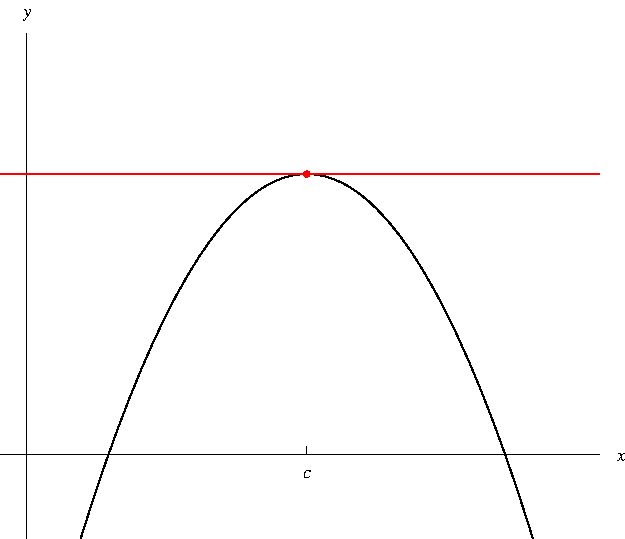
\includegraphics[height=3.5cm]{curve-sketching/pictures/04-03-secondderiv.pdf}%
\column{.7\textwidth}
\begin{itemize}
\item  $f'(c) = 0$, so $f$ has a horizontal tangent at $c$.
\item  $f''(c) < 0$, so $f$ is concave down near $c$.
\item  This means $f$ lies below its horizontal tangent.
\item  This means $f(c)$ is a local maximum.
\end{itemize}
\end{columns}
}%
\end{frame}
% end module second-derivative-test
